\section{Introduction}

This chapter presents the description of the system developed.
The proposed solution implements a software capable of tracking the user's hands and learning and recognizing the objects that are hand-held. 
\\

The name of the project, OCULAR is an acronym of "On-line objeCt Learning And Recognition". 
The first word, on-line, refers to the fact that the learning of new objects is done in real time, there is no need of a training phase in which the software is not operative. 
The logo of the project may be seen in figure \ref{ocular_logo}.
\\

\begin{figure}[H]
	\begin{center}
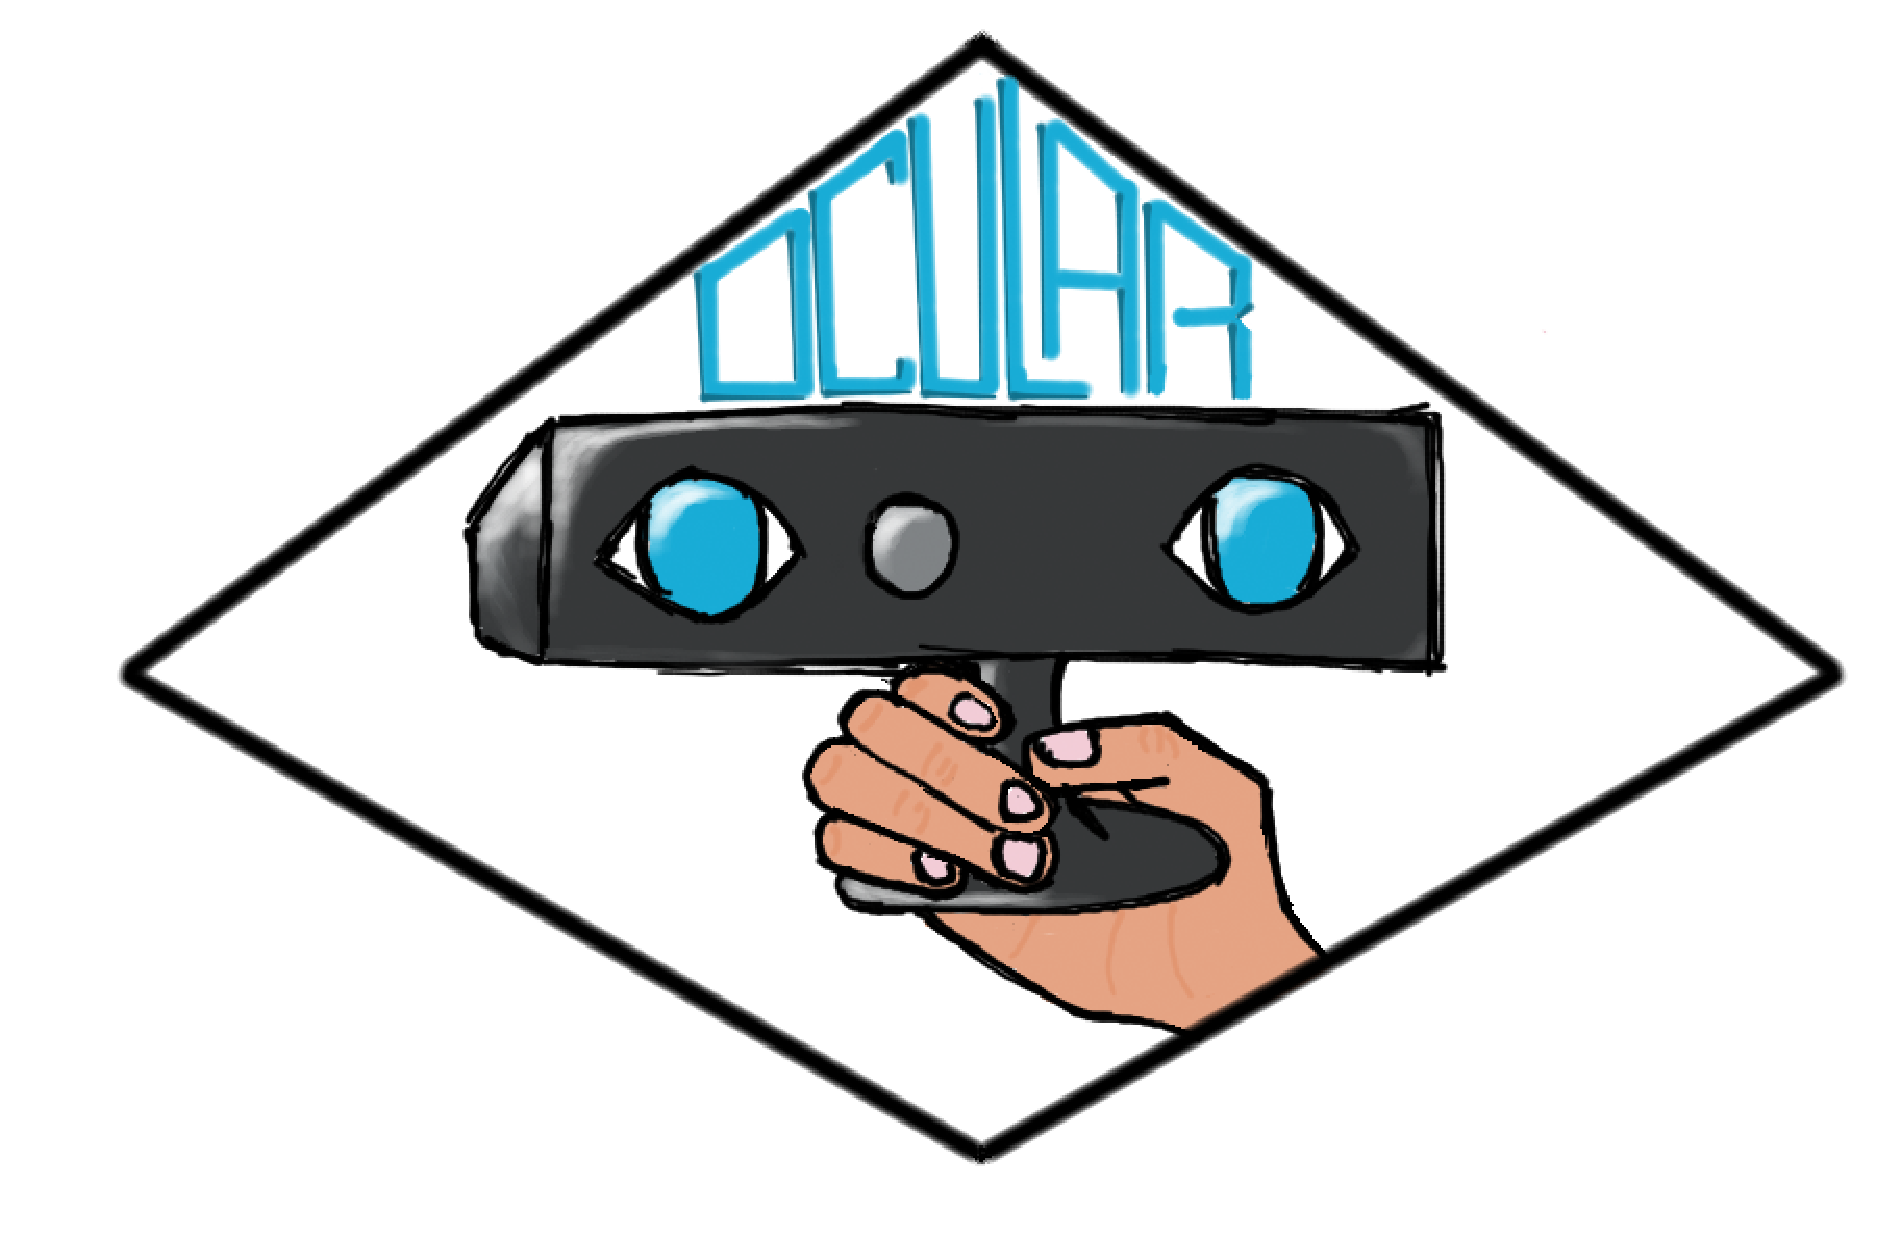
\includegraphics[scale=0.3]{img/ocular_logo.eps}
	\caption[OCULAR Logo]{OCULAR logo}
	\end{center}
	\label{ocular_logo}
\end{figure}

The project's software is modular and the processing has been distributed among different processes.
Those processes are called nodes.  
The Robotic Operating System (ROS) framework has been used in order to improve the communication between nodes and the overall performance of the code. The Point Cloud Library (PCL) and 
the Open Source Computer Vision (OpenCV) C++ libraries have been used in the project to enable 3D and 2D data processing, respectively. 
\\
The following sections are devoted to the design alternatives and the description of the final design used in the project. 